\chapter{Capture et analyse des besoins}

\section{R\^oles}

\begin{description}
    \item[ABADIE Guillaume] Concepteur / D\'eveloppeur
    \item[BUISSON Nicolas] Concepteur / D\'eveloppeur
    \item[CREPET Louise] Concepteur / D\'eveloppeur
    \item[DOMINGUES R\'emi] Chef de projet / Concepteur / D\'eveloppeur
    \item[MARTIN Aline] Responsable qualit\'e / Concepteur / D\'eveloppeur
    \item[WETTERWALD MARTIN] Responsable Git / Concepteur / D\'eveloppeur
\end{description}

\section{Planning pr\'evisionnel du projet}

\begin{landscape}
\begin{figure}[h]
    \centering
    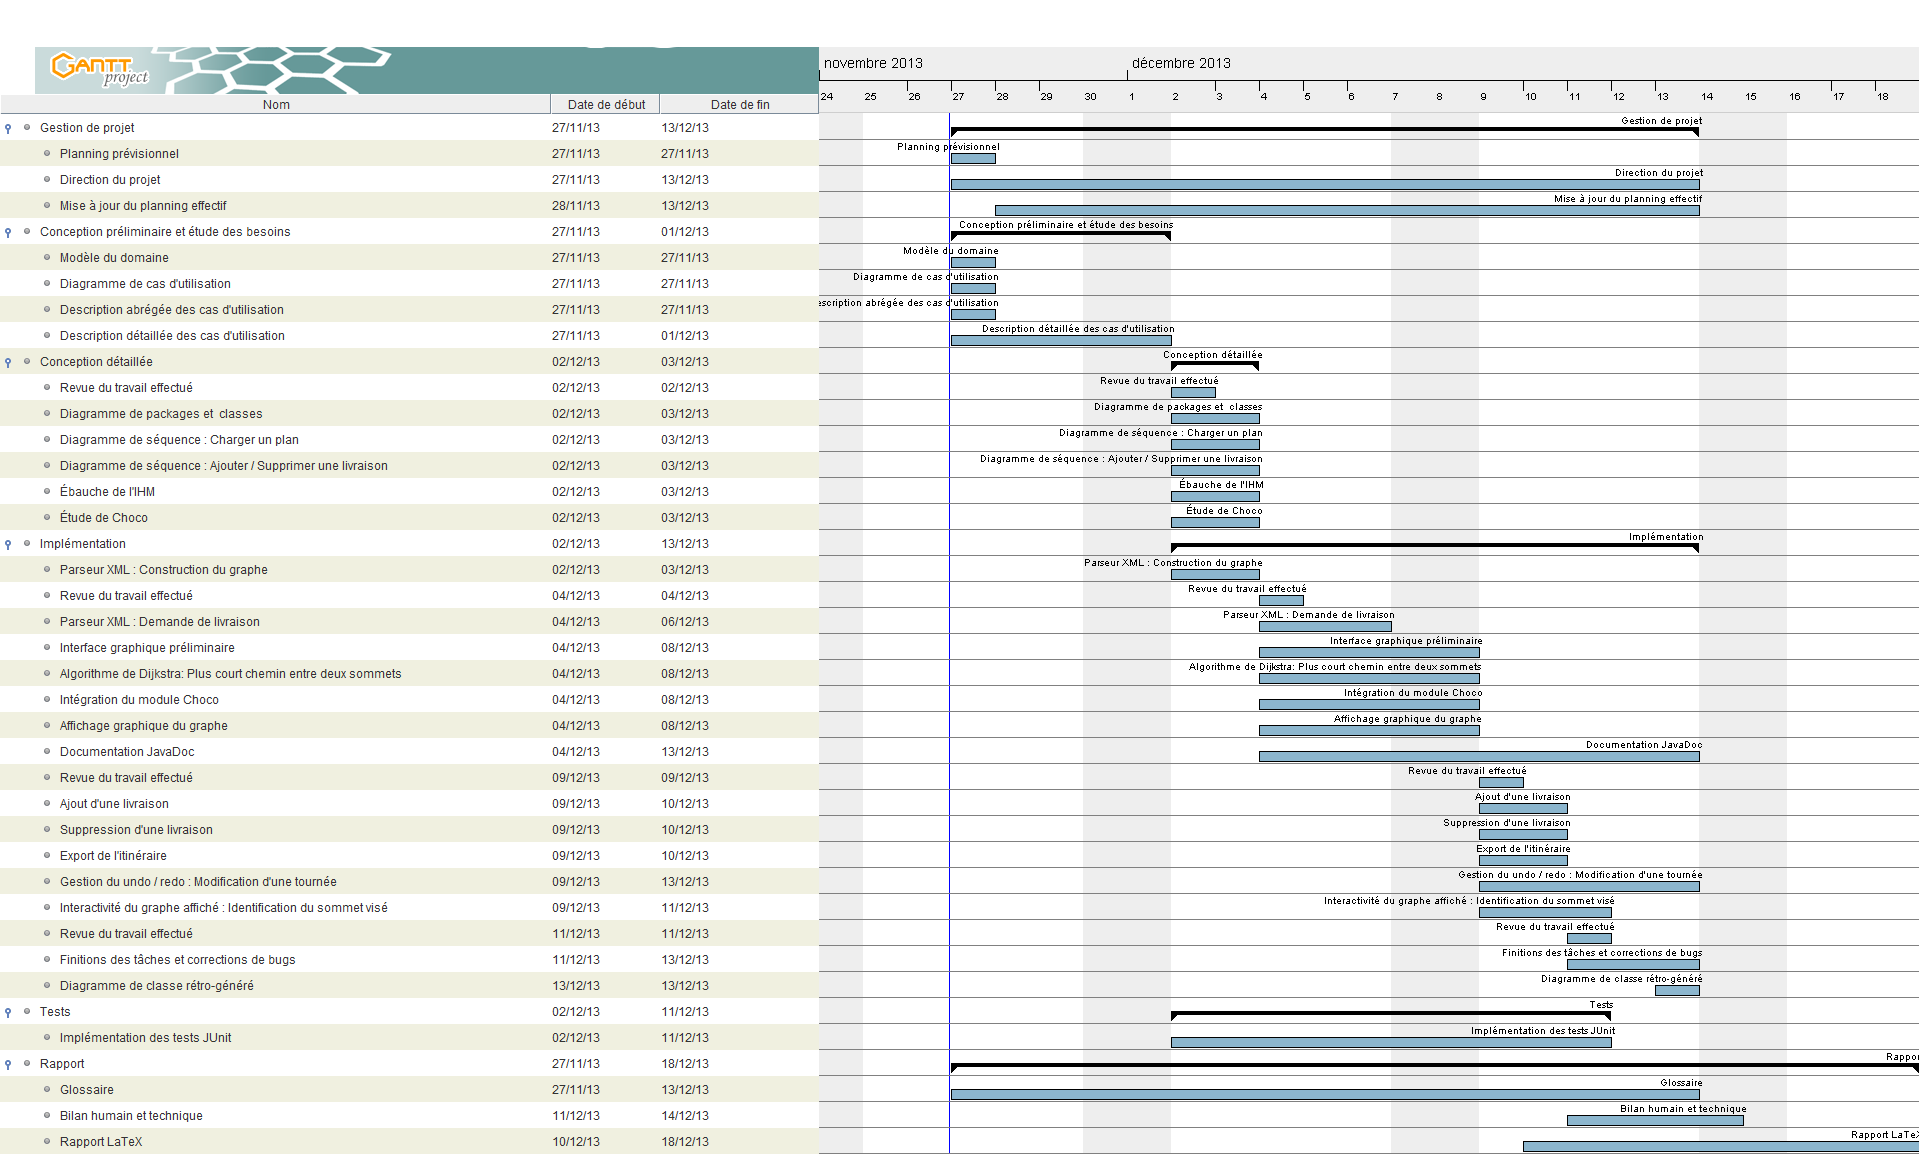
\includegraphics[width=240mm]{../diagrams/project_management/planning_previsionnel/planning_previsionnel.png}
    \caption{Planning pr\'evisionnel du projet}
    \label{diagram:planning_prevision}
\end{figure}
\end{landscape}
\pagebreak


\section{Mod\`ele du domaine}

\begin{figure}[h]
    \centering
    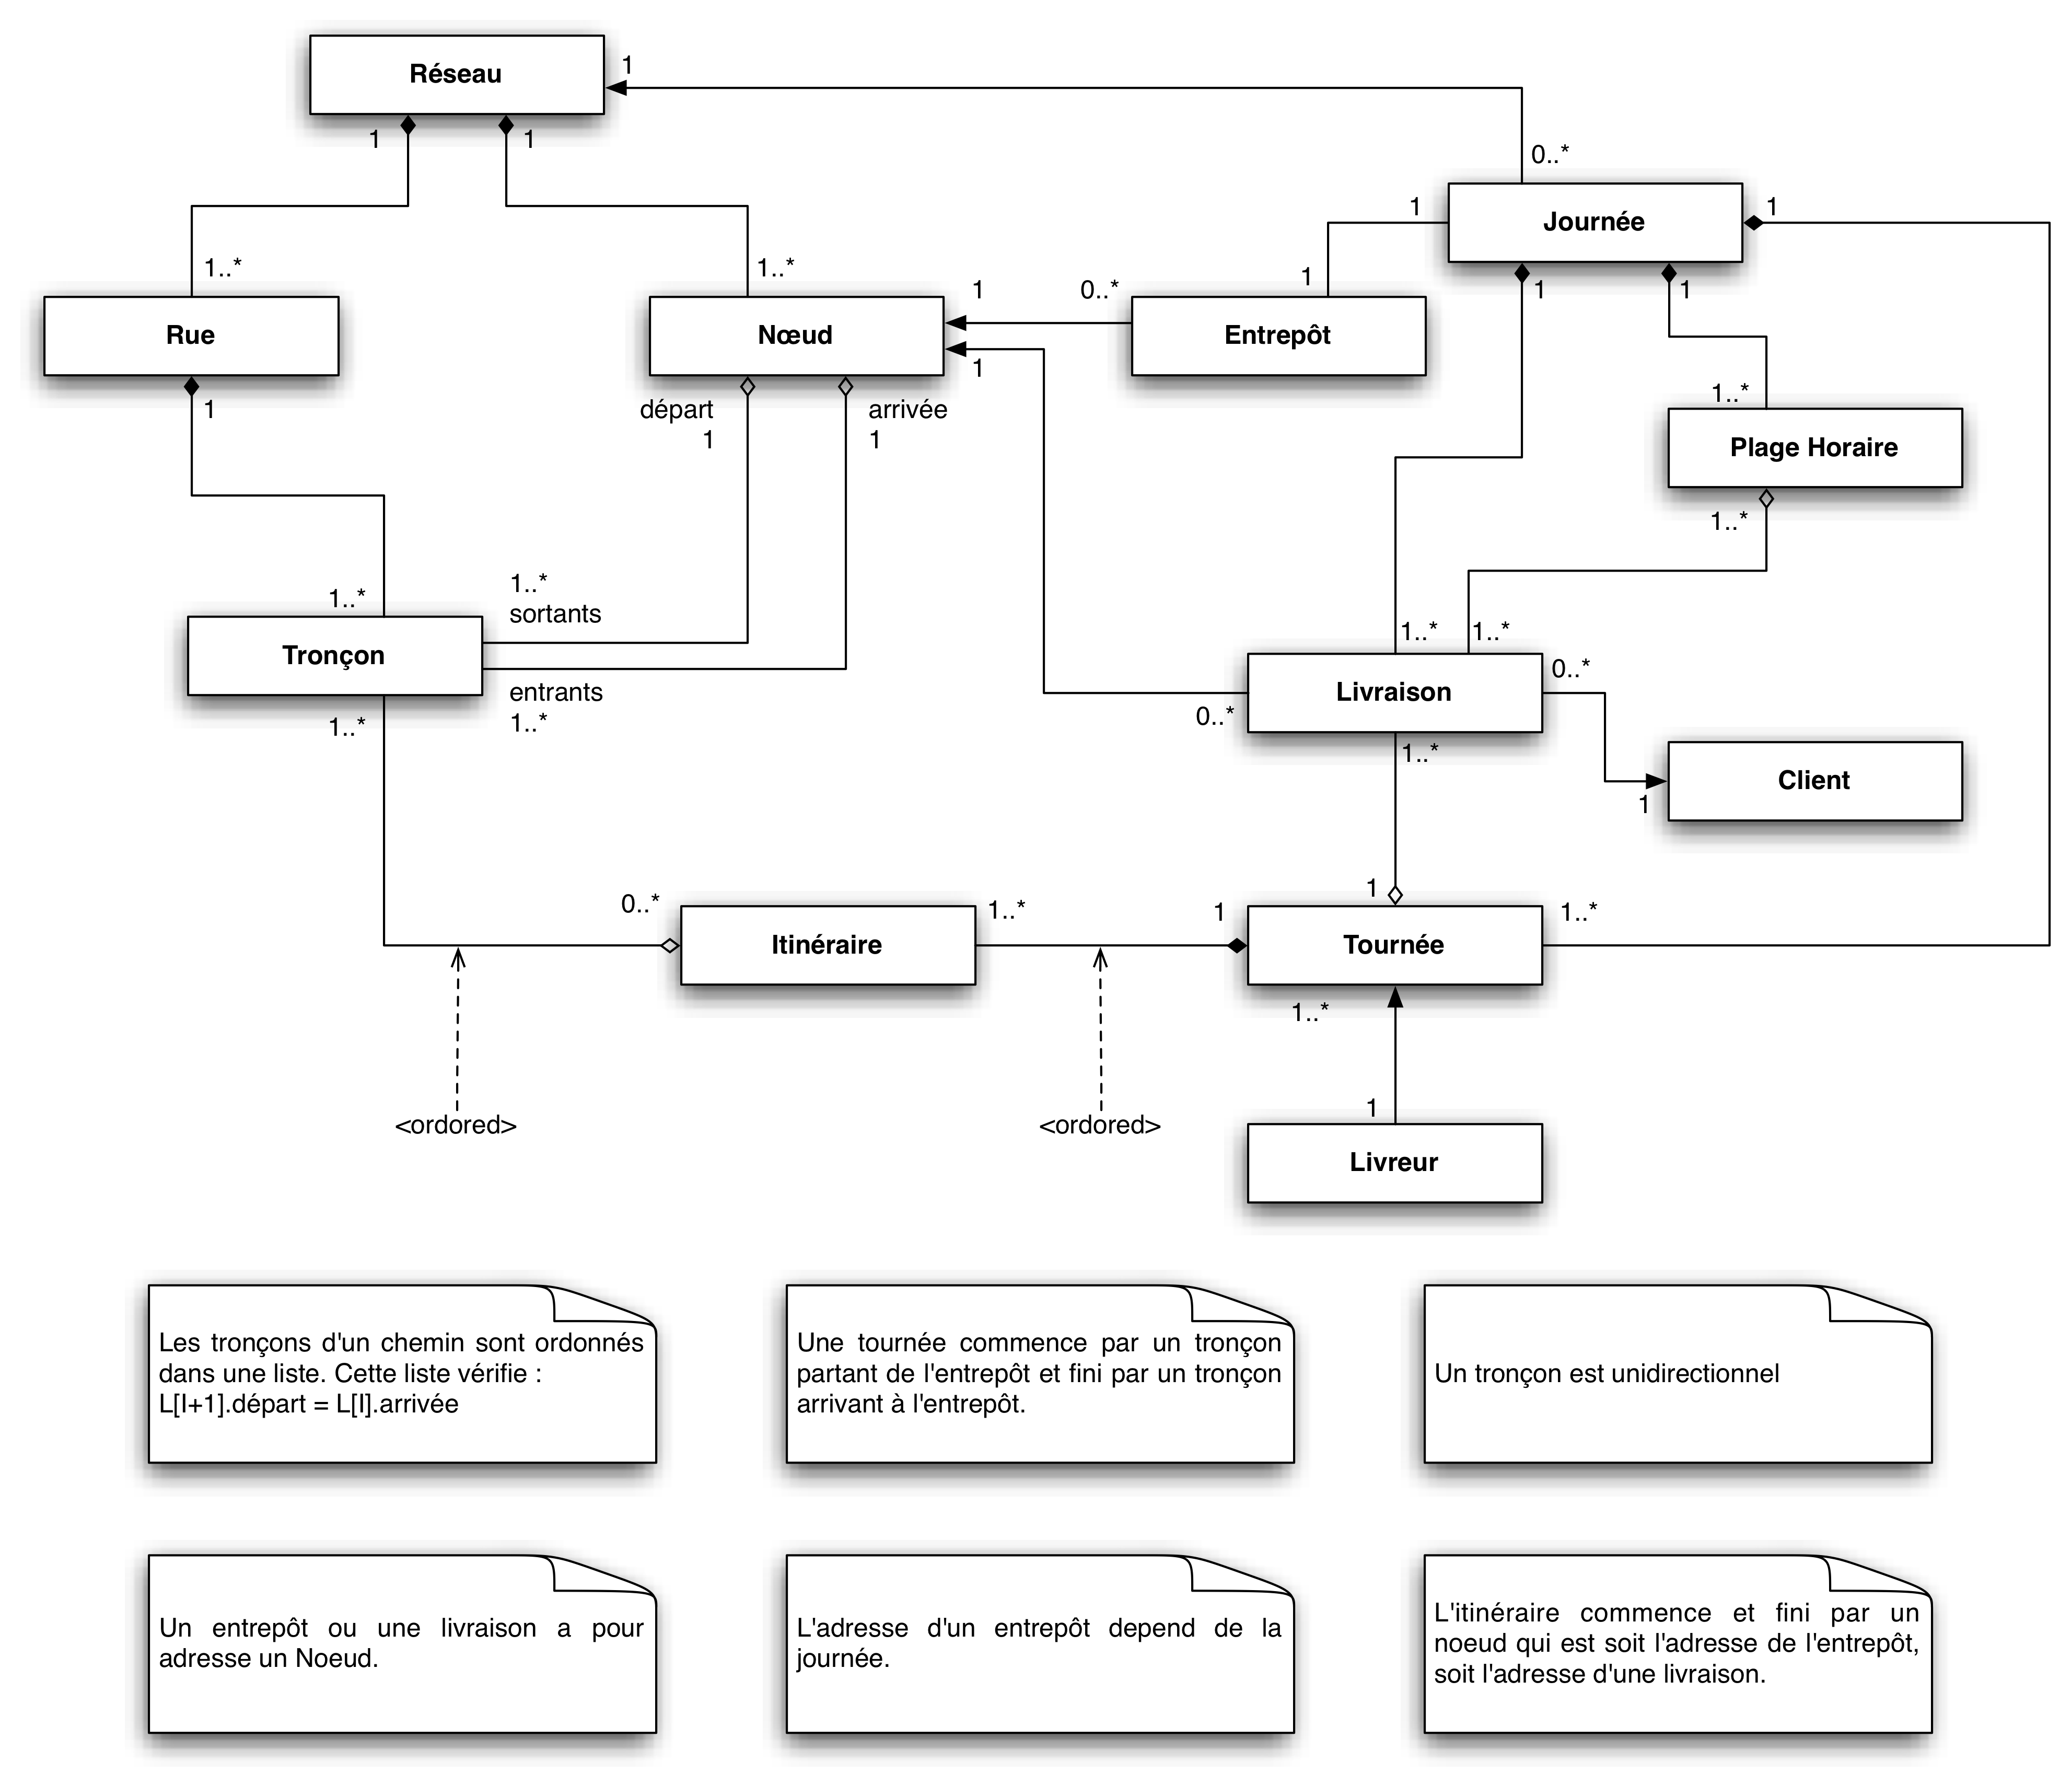
\includegraphics[width=140mm]{../diagrams/domain_model/domaine.png}
    \caption{Mod\`ele du domaine}
    \label{diagram:domaine}
\end{figure}

\pagebreak
\section{Diagramme de cas d’utilisation}

\begin{figure}[h]
    \centering
    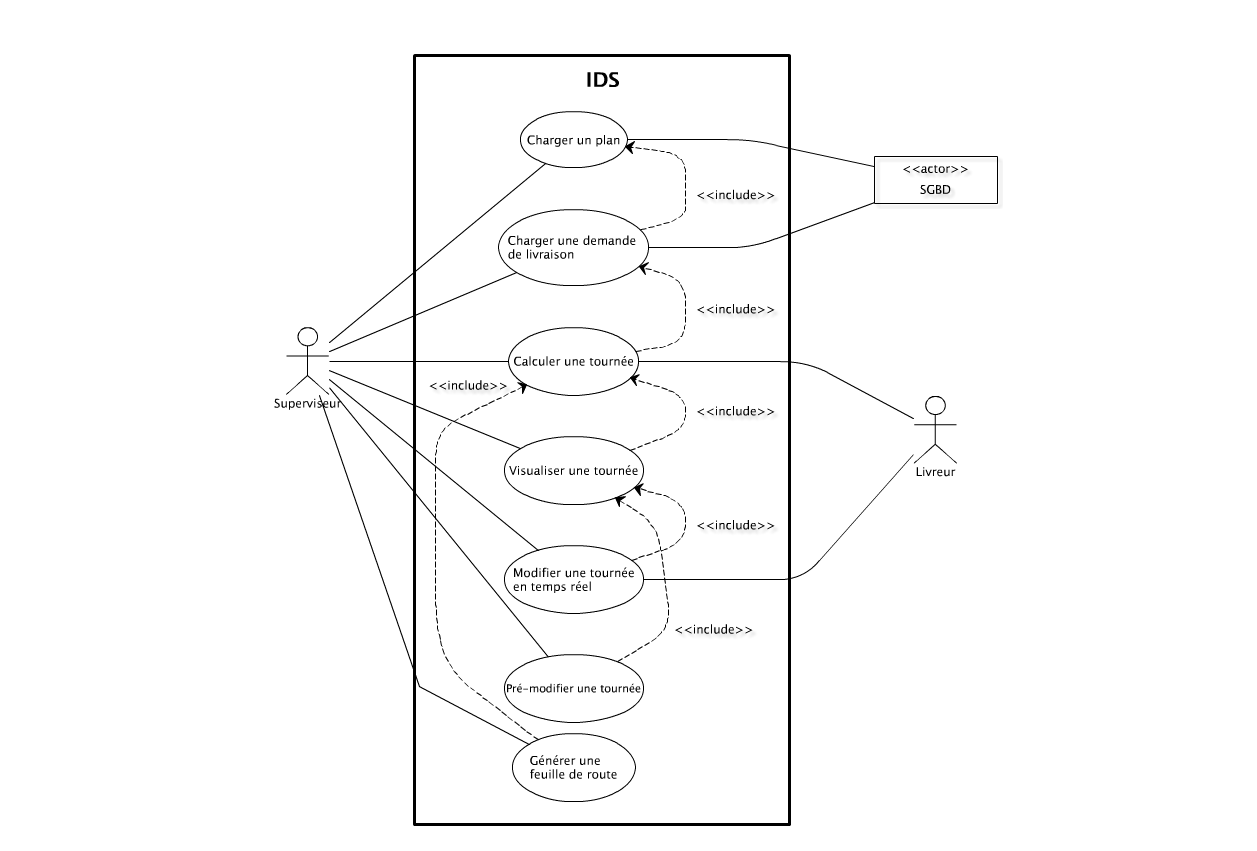
\includegraphics[width=140mm]{../diagrams/use_case/use_case_diagram.png}
    \caption{Diagramme de cas d’utilisation}
    \label{diagram:use_case}
\end{figure}

\section{Description abr\'eg\'ee des cas d’utilisation}

Le système doit permettre plusieurs ensembles d’actions~:

\begin{itemize}
    \item Le superviseur peut à tout moment visualiser le plan d’une zone de la ville, il peut alors y voir les
    points de livraison de la zone, ainsi que leur détails (adresse, état de livraison, etc …).

    \item D’autre part, il peut charger une demande de livraison, celle ci est ajoutée au système et sera traitée
    dans les futures tournées.

    \item Enfin il peut générer une feuille de route multi-support (papier et électronique) à la destination d’un
    des livreurs. Pour cela il peut demander au système de calculer une tournée, et de la visualiser sur un plan.
    Il peut alors y faire d’éventuelles modifications avant la génération de la feuille et lancer cette dernière.

    \item Une fois la feuille de route générée, le superviseur pourra à tout moment modifier une tournée en cours.
    Le livreur de cette tournée modifiée en sera alors informé par le système.
\end{itemize}

